\documentclass[aspectratio=169]{beamer}
\usetheme{Madrid}

\title{Modern Course Design and CS Materials}
\subtitle{}
\author{Kalpathi Subramanian$^1$, Erik Saule$^1$, Jamie Payton$^2$\\\texttt{krs@uncc.edu}, \texttt{esaule@uncc.edu}, \texttt{payton@temple.edu} }
\institute{$^1$The University of North Carolina at Charlotte\\$^2$Temple University}
\date{BRIDGES Workshop, May 30-June 1, 2023}
\setbeamertemplate{footline}

\usepackage{hyperref,graphicx}
\usepackage{subfloat}

\beamertemplatenavigationsymbolsempty % remove navigation symbols
\begin{document}


\begin{frame}
\titlepage
\end{frame}


\AtBeginSection[]
{
    \begin{frame}
        \frametitle{Table of Contents}
        \tableofcontents[currentsection]
    \end{frame}
}


\section{Modern Course Design}

\subsection{High level view}

\begin{frame}
  \frametitle{High Level Picture}

  \begin{columns}
    \column{.45\linewidth}
    \begin{block}{Structured in Module}
      Content is grouped themes

      Dependencies between modules

      \begin{itemize}
      \item Catch up modules
      \item Mandatory Modules
      \item Optional Modules
      \end{itemize}
      
    \end{block}

  \begin{block}{Goals}
    \begin{itemize}
    \item Topics
    \item Course Learning Outcomes
    \item Program Learning Outcomes
    \item Competencies
    \item Pedagogical Strategies
    \end{itemize}
  \end{block}

  \column{.45\linewidth}
  
  \begin{block}{A Variety of Content}
    \begin{itemize}
    \item Lectures
    \item Videos
    \item In-class activities
    \item Assignments
    \item Exam
    \item Projects
    \end{itemize}
  \end{block}


  \begin{block}{Accreditation}
    \begin{itemize}
    \item SACS
    \item ABET
    \item Quality Matters
    \item \textit{insert your accreditation body here}
    \end{itemize}
  \end{block}
  \end{columns}
  
\end{frame}

\subsection{Principles of Alignment}

\begin{frame}
  \frametitle{What is Alignment?}

  \begin{block}{Properties of how content flow in}
    \begin{itemize}
    \item Program
    \item Course
    \item Module
    \item Materials
    \end{itemize}
  \end{block}

  \begin{block}{That could apply to}
    \begin{itemize}
    \item Topics
    \item Outcomes
    \item Competencies
    \end{itemize}
  \end{block}

  \begin{block}{That could be in term of}
    \begin{itemize}
    \item What they cover
    \item What they assume students know
    \end{itemize}
  \end{block}
  
\end{frame}

\begin{frame}
  \frametitle{Aligning Modules with Course Objectives}
    Courses usually have objectives that come from program
    descriptions and assessments.

    How do we ensure that the content of the class actually serve
    these higher objective? We want to align the objective modules
    with the objective of the course.

    Two main properties to check:
    \begin{itemize}
    \item Are all the course objectives covered appropriately by a module objective?
    \item Are there module objectives that serve no course objective?
    \end{itemize}
\end{frame}

\begin{frame}
  \frametitle{Alignment within Module}

  \begin{block}{Typical module structure}
    \begin{itemize}
    \item Exposition to new concept (lecture, textbook, videos)
    \item Clarification of concept (discussion, hands-on activity)
    \item Reinforcement of concept (problem, programming assignment)
    \end{itemize}
  \end{block}
  
  \begin{block}{Properties you want}
    \begin{itemize}
    \item The clarification should not introduce new concepts
    \item The reinforcement should strengthen the exposition and clarification topics
    \item The materials should cover the topics the module is meant to cover
    \item The materials should not wander too far from the module objectives
    \end{itemize}
  \end{block}

  \begin{block}{Assessment}
    Exam should \textbf{never} introduce new concepts
  \end{block}  
\end{frame}

\begin{frame}
  \begin{columns}
    \column{.45\linewidth}
    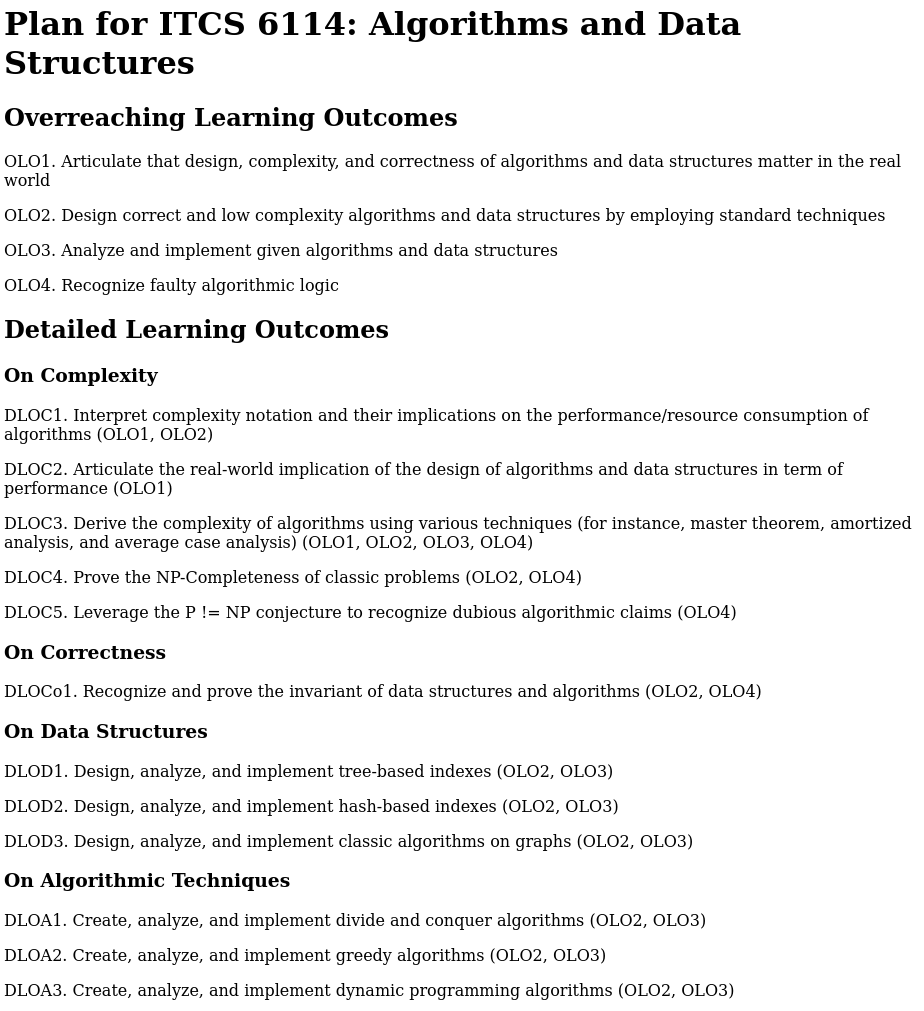
\includegraphics[width=\linewidth]{structure_figs/LOmap.png}
    
    \column{.45\linewidth}
    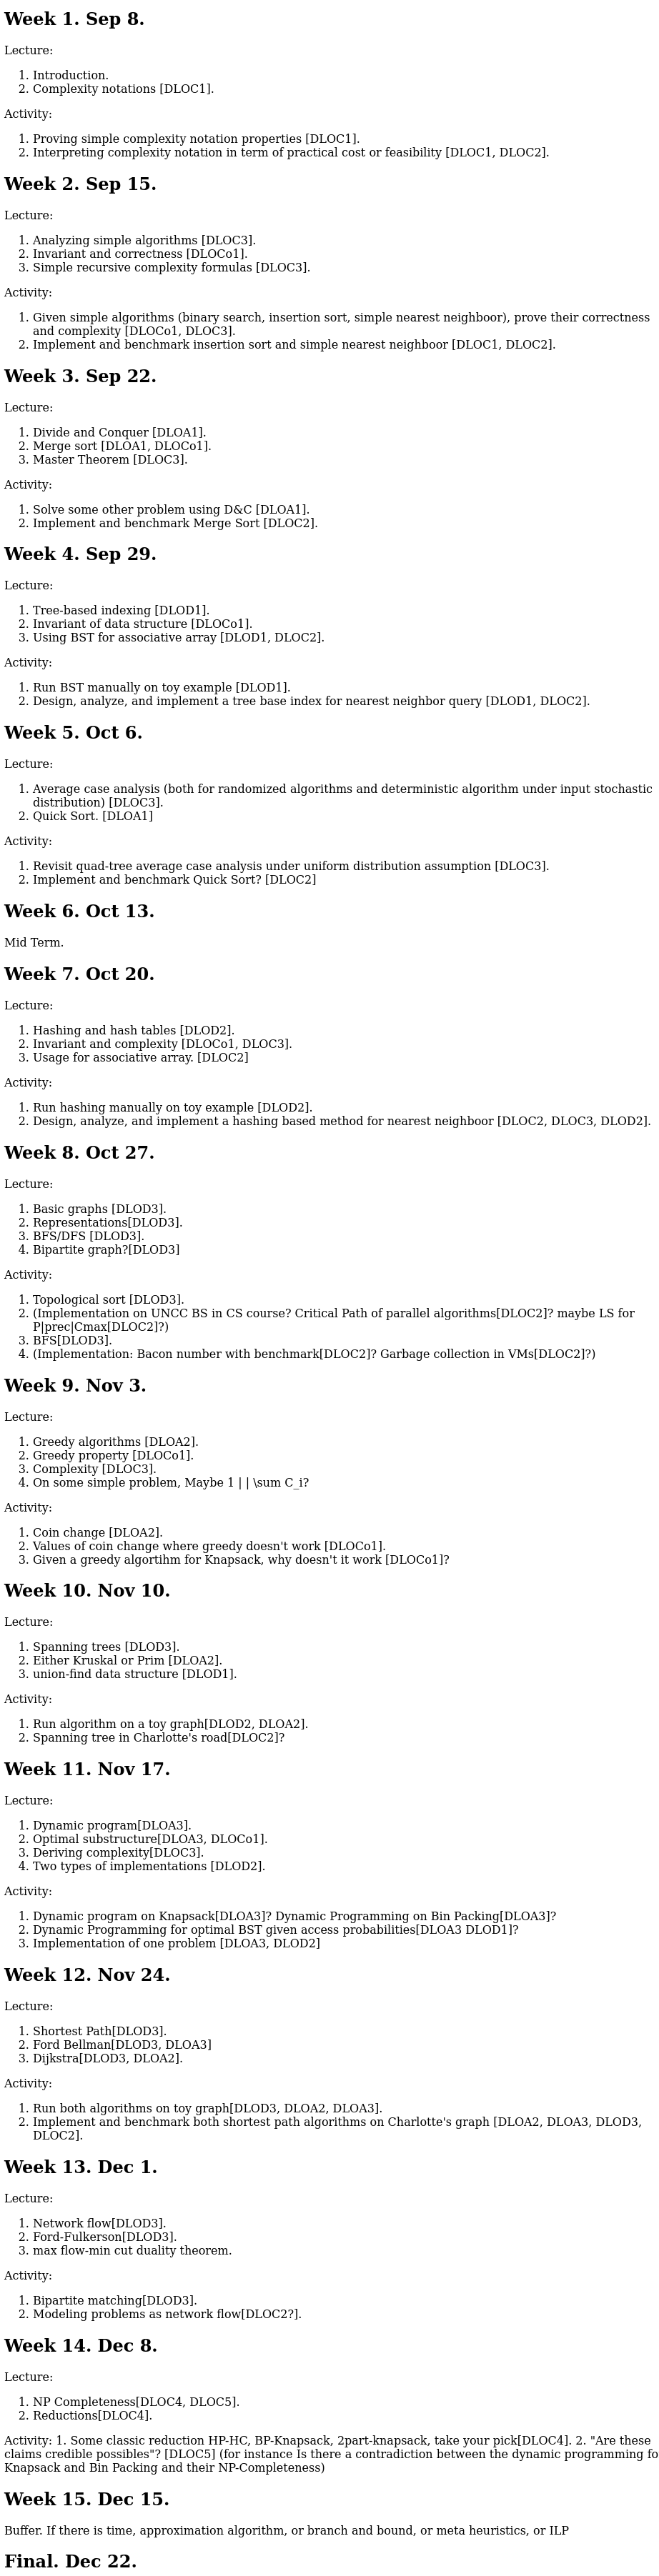
\includegraphics[width=\linewidth, trim=0in 35in 0in 0in, clip]{structure_figs/AgendaMap.png}
    
  \end{columns}
\end{frame}

\subsection{Curriculum Guidelines}


\begin{frame}
  \frametitle{Curriculum Guidelines}

  \begin{block}{What are they?}
    Usually they are recommendation of what should/could be taught across a program.

    Expressed in term of topics, learning outcome, and competencies. Not in term of courses.

    Usually make recommendation on how much one should learn in a
    particular topic, sometimes specified in number of hours.
  \end{block}


  \begin{block}{How can we use them?}
    Give us a reference of what we should/could be teaching.

    Am I covering all that? Should I? Why not?

    Give us a common language to communicate between instructors.
  \end{block}
\end{frame}

\begin{frame}
  \frametitle{General Guidelines: ACM/IEEE CS 2013}

  \begin{columns}
    
    \column{.45\linewidth}
    
  Structured in
  \begin{itemize}
  \item Knowledge Area
  \item Knowledge Unit
  \end{itemize}

  Topics and Learning Outcomes are classified as
  \begin{itemize}
  \item Tier-1
  \item Tier-2
  \item Elective
  \end{itemize}
  
  Other general guidelines:
  \begin{itemize}
  \item Data Science
  \item Computer Engineering
  \item Upcoming revised CS
  \end{itemize}
  
    \column{.53\linewidth}
    
  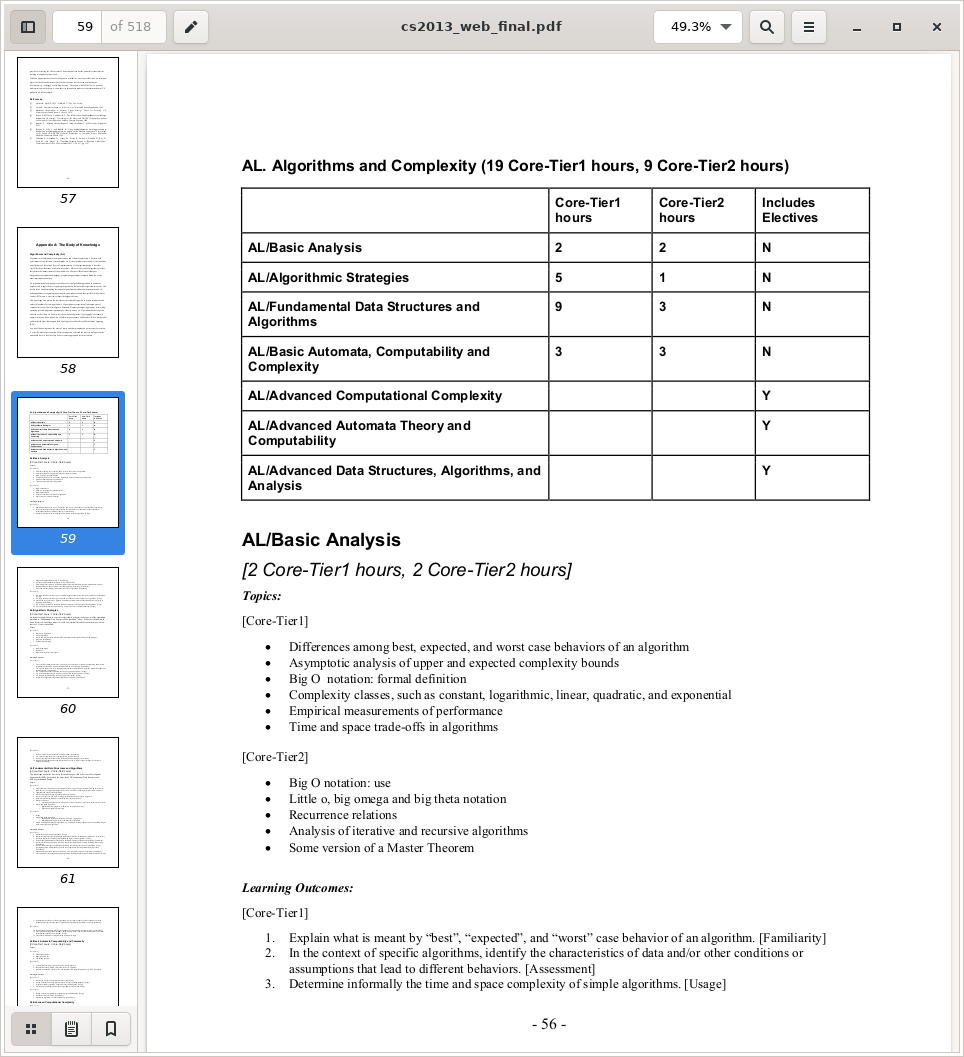
\includegraphics[width=\linewidth]{figs/cs2013-ALpage1.png}

  \end{columns}
\end{frame}

\begin{frame}
  \frametitle{Specific Guidelines: NSF/IEEE-TCPP PDC 2012}

  Structured in domains:
  \begin{itemize}
  \item Programming
  \item Algorithm
  \item Architecture
  \end{itemize}

  More descriptive.

  Bloom levels.

  Other specific guidelines: graphics, security  
\end{frame}


\begin{frame}
  \frametitle{A Lingua Franca}

  CS Guidelines give us a fairly detailed description of what is in CS.

  We can use them as ontologies to describe in a common language what
  a course of a class material is like.

  \begin{block}{What do you think is in a lecture entitled UNCC-ITCS-2214-Saule-Graphs?}
    \tiny
  \begin{itemize} 
    \item Depth- and breadth-first traversals
    \item Representations of graphs (e.g., adjacency list, adjacency matrix)
    \item Reflexivity, symmetry, transitivity
    \item Illustrate by example the basic terminology of graph theory, and some of the properties and special cases of each type of graph/tree.
    \item Undirected graphs
    \item Directed graphs
    \item Weighted graphs
    \item Iterative and recursive traversal of data structures
  \end{itemize}
  \end{block}
\end{frame}

\begin{frame}
  \frametitle{CS material pitch}
\end{frame}

\end{document}
%
